% Бүлэг 1

\chapter{Онолын ойлголт} % Бүлгийн нэр
\label{Chapter1} % Энэ бүлэг рүү ишлэл хийх бол \ref{Chapter1} командыг ашигла 

%-------------------------------------------------------------------------------

% Агуулгад ашигласан хэвшүүлэлтийн зарим командын тодорхойлолт
\newcommand{\keyword}[1]{\textbf{#1}}
\newcommand{\tabhead}[1]{\textbf{#1}}
\newcommand{\code}[1]{\texttt{#1}}
\newcommand{\file}[1]{\texttt{\bfseries#1}}
\newcommand{\option}[1]{\texttt{\itshape#1}}


%-------------------------------------------------------------------------------
\section{Ерөнхий ойлголт}
Орчин үеийн цахим үйлчилгээний салбарт хууль зүйн зөвлөгөө, мэдээллийн хүртээмжийг нэмэгдүүлэх нь нийгмийн болон технологийн тулгамдсан асуудал болоод байна. Мэдээллийн системийн хувьсал болон хиймэл оюуны хөгжлийн үр дүнд хуулийн нарийн төвөгтэй бичвэрийг боловсруулах, шинжлэх, иргэдэд ойлгомжтой хэлбэрт шилжүүлэх боломж бүрдэж байна.

Хууль зүйн салбарт энэхүү хандлага эрчимжиж байгаа нь иргэдийн хууль эрх зүйн боловсролыг дэмжих, баталгаатай эх сурвалжаас шуурхай мэдээлэл авах хэрэгцээг хангах ухаалаг системийн шаардлагыг бий болгож байна. Ийм систем нь хэрэглэгчийн асуултад хариу өгөхөөс гадна, мэдээллийн санд буй албан ёсны эх сурвалжид тулгуурлан шийдвэр гаргалтад дэмжлэг үзүүлэх (Decision Support) чухал хэрэгсэл юм.

Хиймэл оюунд суурилсан эрх зүйн зөвлөх систем нь хууль зүйн мэдлэгийг олон нийтэд хүртээмжтэй болгох, төрийн үйлчилгээний ачааллыг бууруулах, иргэдийн хууль ёсны эрхийг хамгаалахад технологийн давуу талыг ашиглан бодит хувь нэмэр оруулах боломжийг нээж өгч байна.

%-------------------------------------------------------------------------------

\section{Төслийн ажлын зорилго}

Энэхүү төслийн ажлын ерөнхий зорилго нь Монгол Улсын иргэдэд хууль эрх зүйн мэдээллийг хүртээмжтэй, ойлгомжтой, бодит эх сурвалжид тулгуурлан шуурхай хүргэх зорилготой ``хиймэл оюунд суурилсан эрх зүйн цахим зөвлөх системийг'' хөгжүүлэх явдал юм.

Төслийн ажлын тодорхой зорилтуудыг дараах байдлаар тодорхойлов:

\begin{enumerate}
    \item Монгол Улсын хууль зүйн зах зээлийн одоогийн байдал, иргэдийн хууль зүйн үйлчилгээ авах эрэлт, нийлүүлэлтийн зөрүүг шинжилж, дижитал шийдлийн шаардлагыг тодорхойлох;

    \item Хууль зүйн мэдээллийг бүтэцжүүлэн хадгалах, мэдээлэл сэргээн нөхөн авах болон генерацлах зарчим (Retrieval-Augmented Generation, RAG)-д суурилсан мэдээлэл сэргээх механизм бүхий системийн архитектурыг зохион бүтээх;

    \item FastAPI, PostgreSQL, Next.js болон Google Gemini 2.5 Flash загварыг ашиглан backend, frontend болон хиймэл оюуны интеграцчилалтай, модульчлагдсан, өргөтгөх боломжтой вэб системийг хөгжүүлэх;

    \item Системийн аюулгүй байдал, өгөгдлийн нууцлал, хариу өгөх хурдыг хангах техникийн шийдлүүдийг хэрэгжүүлэх;

    \item Хэрэглэгчийн шаардлагад нийцүүлэн ерөнхий иргэн, хуульч, админ гэсэн үндсэн оролцогч талуудын ашиглалтын хувилбаруудыг тодорхойлж, use case, дарааллын диаграм, ERD зэрэг загварчлалуудыг боловсруулах;

    \item Хөгжүүлсэн системийн үр дүнг туршиж, хууль зүйн зөвлөгөөний чанар, хүртээмж, хэрэглэхэд хялбар байдлыг үнэлэх.
\end{enumerate}

Эдгээр зорилтуудыг биелүүлснээр Монгол Улсад хууль зүйн боловсролыг дэмжих, төрийн үйлчилгээний ачааллыг бууруулах, иргэдийн хууль ёсны эрхийг хамгаалахад орчин үеийн технологид суурилсан бодит шийдэл бий болно.

%-------------------------------------------------------------------------------

\section{Монгол Улсын хууль зүйн зах зээлийн судалгаа}

Монгол Улсад хууль зүйн үйлчилгээний салбар нь "Дижитал Монгол" хөтөлбөрийн хүрээнд эрчимтэй цахимжиж байна. 2025 оны эцсийн статистик мэдээллээр Монгол Улсын интернет хэрэглэгчдийн тоо 3.1 саяд хүрч, хүн амын 92.4 хувийг хамарсан байна. Энэ нь хиймэл оюунд суурилсан (AI-driven) үйлчилгээг зах зээлд нэвтрүүлэх техникийн дэд бүтэц бүрэн хангагдсаныг илтгэж байна.

%-------------------------------------------------------------------------------
\subsection{Хууль зүйн үйлчилгээний эрэлт ба нийлүүлэлтийн зөрүү}

Өнөөдрийн байдлаар Монголын Хуульчдын Холбоонд бүртгэлтэй 6,400 гаруй хуульч үйл ажиллагаа явуулж байгаа ч иргэдийн хувьд анхан шатны зөвлөгөө авах зардал өндөр (дунджаар нэг цаг нь 50,000төг - 200,000төг) хэвээр байна. 2025 оны "LegalTech" судалгаанаас үзэхэд иргэдийн 76 хувь нь хуулийн асуудлаа эхлээд цахимаар хайж, AI туслахаас чиглүүлэг авах сонирхолтой байгаа нь ажиглагдсан. Гэвч зах зээлд байгаа шийдлүүд нь зөвхөн "текст хайх" (keyword search) түвшинд байгаа нь RAG (Retrieval-Augmented Generation) архитектурт суурилсан ухаалаг системийн орон зайг бий болгож байна.
%-------------------------------------------------------------------------------
\subsection{Зорилтот хэрэглэгчдийн шинжилгээ}

Системийн хэрэглэгчдийг дараах 3 үндсэн сегментэд хуваан авч үзэж болно:

\begin{enumerate}
    \item \textbf{Дижитал иргэд (18-45 нас):} Хуулийн асуудлаа цаг алдалгүй, гар утаснаасаа шийдэхийг эрмэлздэг бүлэг.
    
    \item \textbf{Бичил ба жижиг бизнес эрхлэгчид:} Хуульчийн байнгын зардал гаргах боломжгүй ч гэрээ болон дүрэм журмын анхан шатны чиглүүлэг авах шаардлагатай талууд.
    
    \item \textbf{Хуулийн салбарын оюутнууд:} Хуулийн кейс дээр дүн шинжилгээ хийх, эх сурвалж хайх явцаа хурдасгах зорилготой хэрэглэгчид.
\end{enumerate}
%-------------------------------------------------------------------------------
\subsection{SWOT шинжилгээ}

\begin{enumerate}
    \item \textbf{Давуу тал (Strengths):} 
    RAG технологи: Зөвхөн албан ёсны хуулийн санд тулгуурладаг тул худал мэдээлэл өгөх (hallucination) эрсдэл бага.

    \item \textbf{Сул тал (Weaknesses):} 
    Шийдвэр гаргах эрх зүйн чадамжгүй байдал: Уг систем нь зөвхөн "зөвлөх" болон "мэдээлэл өгөх" зориулалттай бөгөөд бодит шүүхийн шийдвэр гаргах эсвэл өмгөөлөгчийг бүрэн орлох хууль зүйн чадамжгүй. Хэрэглэгч системийн хариултыг эцсийн үнэн гэж хүлээн авах нь эрсдэлтэй бөгөөд энэ нь технологийн бус, хэрэглээний сул тал юм.

    \item \textbf{Боломж (Opportunities):} 
    Хууль зүйн цоорхой: Монголын зах зээлд AI зөвлөх системүүд стандартчилагдаж эхлээгүй байгаа нь ``анхдагч'' болох боломж.

    \item \textbf{Аюул (Threats):} 
    Ёс зүйн зохицуулалт: AI-ийн өгсөн хариултад хариуцлага хүлээх эрх зүйн орчин тодорхойгүй байгаа байдал.
\end{enumerate}
%-------------------------------------------------------------------------------

\section{Ижил төстэй системийн судалгаа}
AI-д суурилсан хуулийн зөвлөх системтэй ижил төстэй гадаад, дотоодын платформууд цөөнгүй байгаа бөгөөд тэдгээр нь хэрэглэгчдэд хууль зүйн мэдээллийг хүргэх, зөвлөгөө өгөх, зарим тохиолдолд шууд хуульчтай холбогдох боломжийг олгодог
%-------------------------------------------------------------------------------
\subsection{Гадаадын системүүдтэй харьцуулсан судалгаа}
\subsubsection{Harvey AI (Дэлхийн тэргүүлэгч Legal AI)}
\paragraph{}
Harvey нь OpenAI-ийн хөрөнгө оруулалттай, зөвхөн хуулийн фирмүүдэд зориулсан хамгийн дэвшилтэт систем юм.

\begin{itemize}
    \item \textbf{Технологийн онцлог:} GPT-4 загварыг хууль зүйн асар том өгөгдлийн сан дээр нэмэлтээр сургасан (fine-tuned). Энэ нь гэрээний шинжилгээ, хуулийн судалгаа, баримт бичиг боловсруулах үйлдлийг өндөр түвшинд гүйцэтгэдэг.

    \item \textbf{Давуу тал:} Маш нарийн төвөгтэй хуулийн логик дүгнэлт хийх чадвартай. ``PwC'', ``Allen \& Overy'' зэрэг дэлхийн топ фирмүүд ашигладаг.

    \item \textbf{Сул тал:} Зөвхөн томоохон байгууллагуудад зориулагдсан (B2B), үнэ өндөр, Монгол хэл болон Монгол Улсын хууль тогтоомжийг дэмждэггүй.
\end{itemize}

\begin{figure}[htbp]
	\centering
	
\includegraphics[scale=0.3]{Chart/HarveyHomePage.png}
	\caption[Harvey нүүр хуудас]{Harvey}
	\label{fig:Chart1}
\end{figure}

\subsubsection{Amberlo (Хуулийн фирмийн удирдлагын цогц систем)}
\paragraph{}

Amberlo бол AI-аас гадна хуулийн фирмийн өдөр тутмын үйл ажиллагааг (Practice Management) автоматжуулдаг систем юм.

\begin{itemize}
    \item \textbf{Технологийн онцлог:} Үүлэн технологид суурилсан (SaaS). Кейс менежмент, цаг бүртгэл, нэхэмжлэх үүсгэх, баримт бичиг хадгалах функцүүдтэй.

    \item \textbf{Давуу тал:} Хуульчдын ажлын бүтээмжийг нэмэгдүүлдэг, хэрэглэхэд хялбар интерфэйстэй. Европ болон дэлхийн олон улсын хууль зүйн стандартад нийцсэн.

    \item \textbf{Сул тал:} Энэ нь ``зөвлөх'' систем гэхээсээ илүү ``удирдлагын'' систем юм. AI-ийн утга зүйн хайлт, зөвлөгөө өгөх чадвар нь Harvey-тай харьцуулахад хязгаарлагдмал.
\end{itemize}

\begin{figure}[htbp]
	\centering
	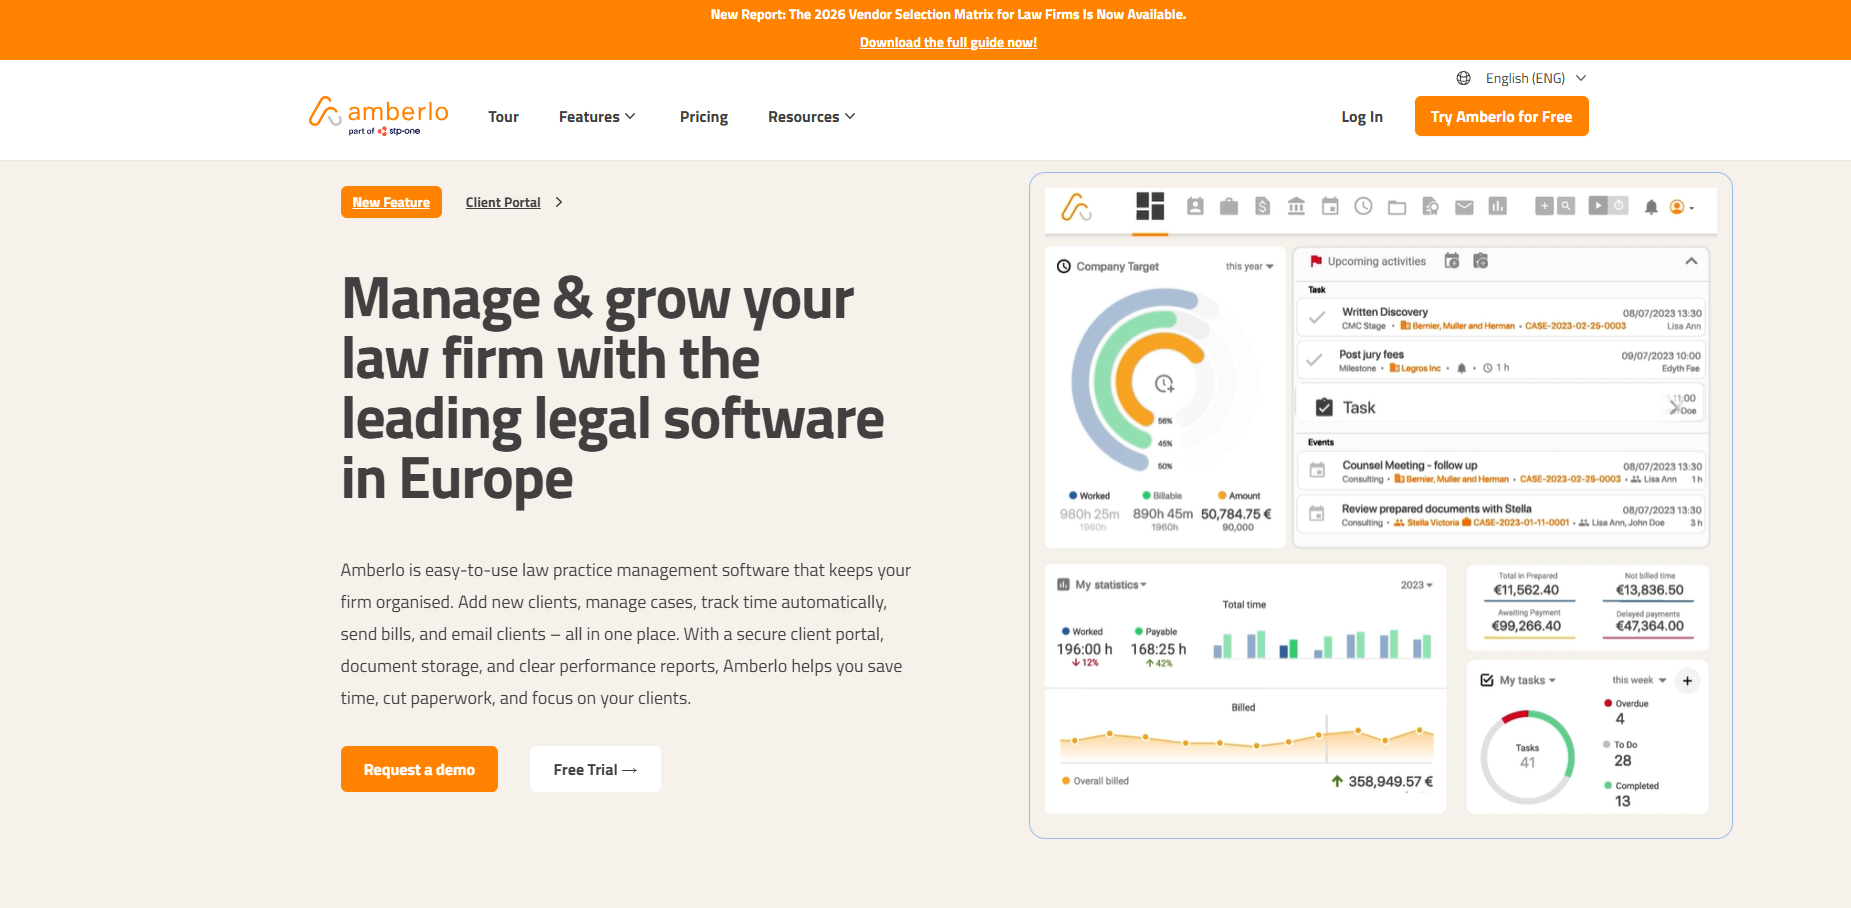
\includegraphics[scale=0.3]{Chart/amberloHomePage.png}
	\caption[Amberlo нүүр хуудас]{Amberlo}
	\label{fig:Chart1}
\end{figure}

\subsection{Монголын системүүдтэй харьцуулсан судалгаа}

\subsubsection{Legalinfo.mn (Эрх зүйн мэдээллийн нэгдсэн систем)}
\paragraph{}
Монгол Улсын бүх шатны хууль тогтоомж, дүрэм журмыг цахим хэлбэрээр хадгалдаг албан ёсны хамгийн том мэдээллийн сан юм.

\begin{itemize}
    \item \textbf{Технологийн онцлог:} Уламжлалт реляци өгөгдлийн сан (SQL) болон түлхүүр үгээр хайх (Keyword search) систем дээр суурилсан.

    \item \textbf{Давуу тал:} Хамгийн сүүлийн үеийн, албан ёсны эх сурвалжтай. Бүх хуулийг файл хэлбэрээр татаж авах боломжтой.

    \item \textbf{Сул тал:} Хэрэглэгч өөрт тохиолдсон асуудалд яг аль хуулийн ямар заалт хамааралтайг өөрөө хайж олох ёстой. Хуулийн хэллэг нь энгийн иргэдэд ойлгоход хэцүү бөгөөд "ухаалаг" зөвлөгөө өгөх функц байхгүй.
\end{itemize}

\begin{figure}[htbp]
	\centering
	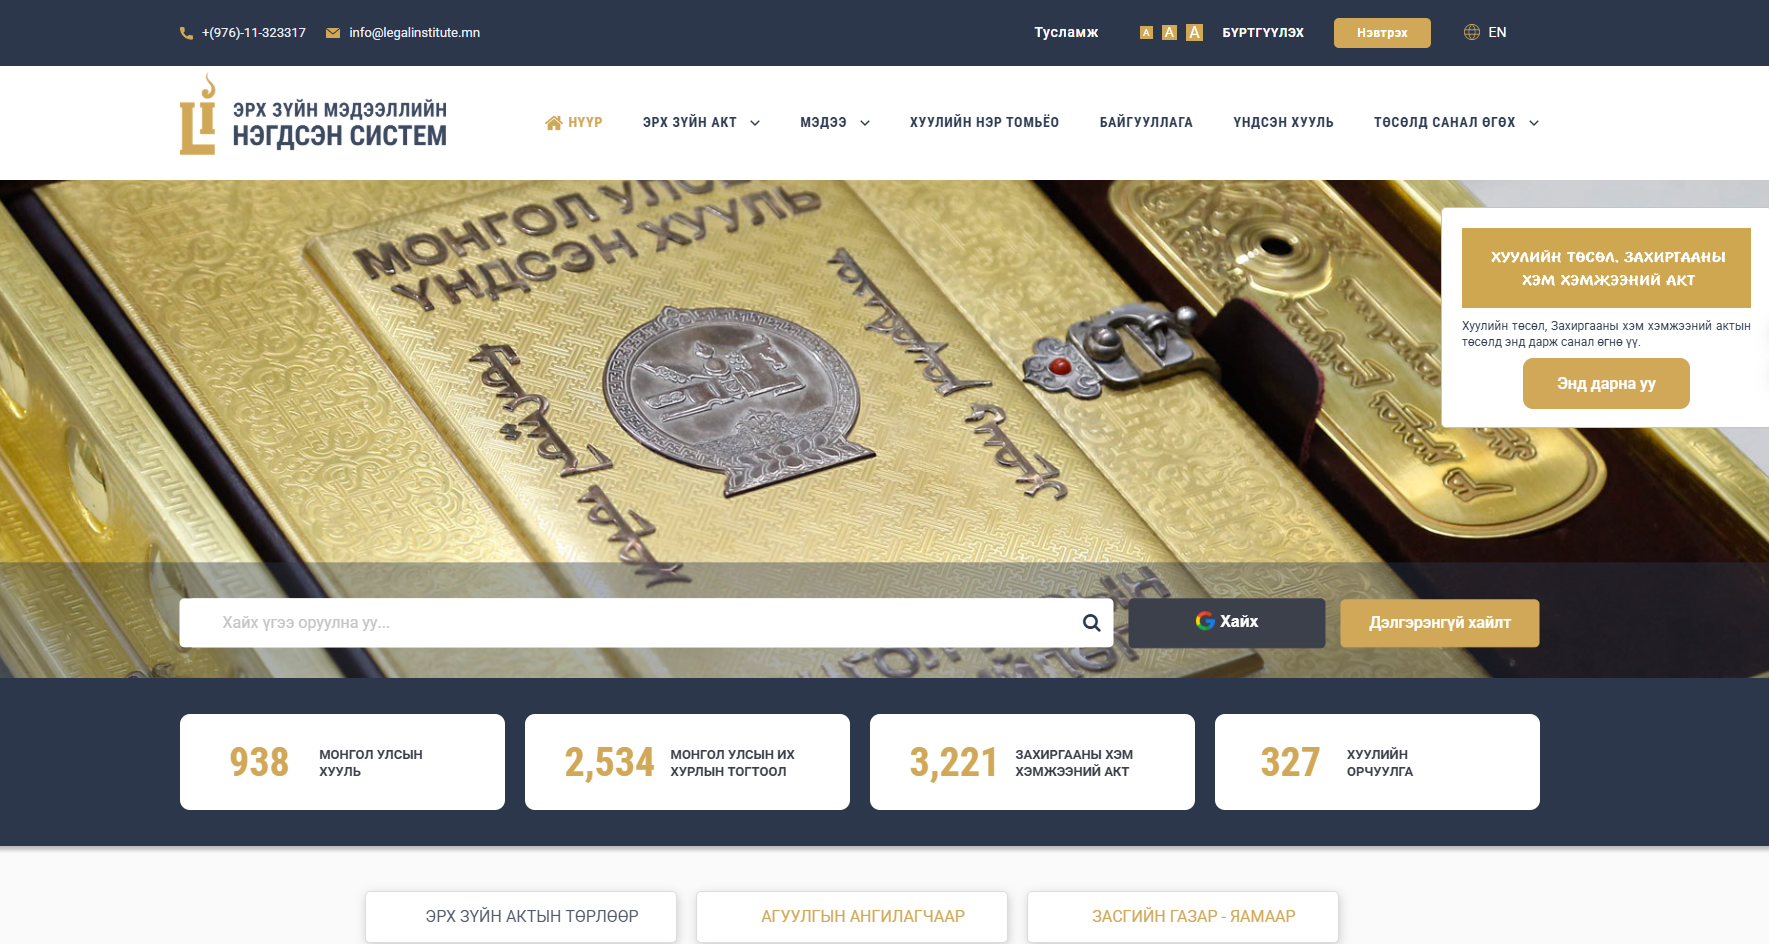
\includegraphics[scale=0.3]{Chart/legalInfo.png}
	\caption[LegalInfo нүүр хуудас]{LegalInfo}
	\label{fig:Chart1}
\end{figure}

\subsubsection{E-khutuch.mn (Эрх зүйн хөтөч)}
\paragraph{}
Иргэдийн эрх зүйн боловсролыг дээшлүүлэх, анхан шатны туслалцаа үзүүлэх зорилготой Хууль зүйн үндэсний хүрээлэнгийн платформ.

\begin{itemize}
    \item \textbf{Технологийн онцлог:} Асуулт-хариултын бэлэн сан (FAQ) болон мэдээллийн нийтлэлүүд дээр суурилсан вэб систем.

    \item \textbf{Давуу тал:} Гэр бүл, өв залгамжлал, хөдөлмөр гэх мэт чиглэлээр түгээмэл тохиолддог асуудлуудад бэлэн хариулт өгдөг. Энгийн иргэдэд зориулсан гарын авлага ихтэй.

    \item \textbf{Сул тал:} Хязгаарлагдмал бэлэн өгөгдөл дээр суурилдаг. Хэрэглэгч өөрийн өвөрмөц кейсийг бичээд хариулт авах боломжгүй (Статик систем). Хиймэл оюуны боловсруулалт байхгүй.
\end{itemize}

\begin{figure}[htbp]
	\centering
	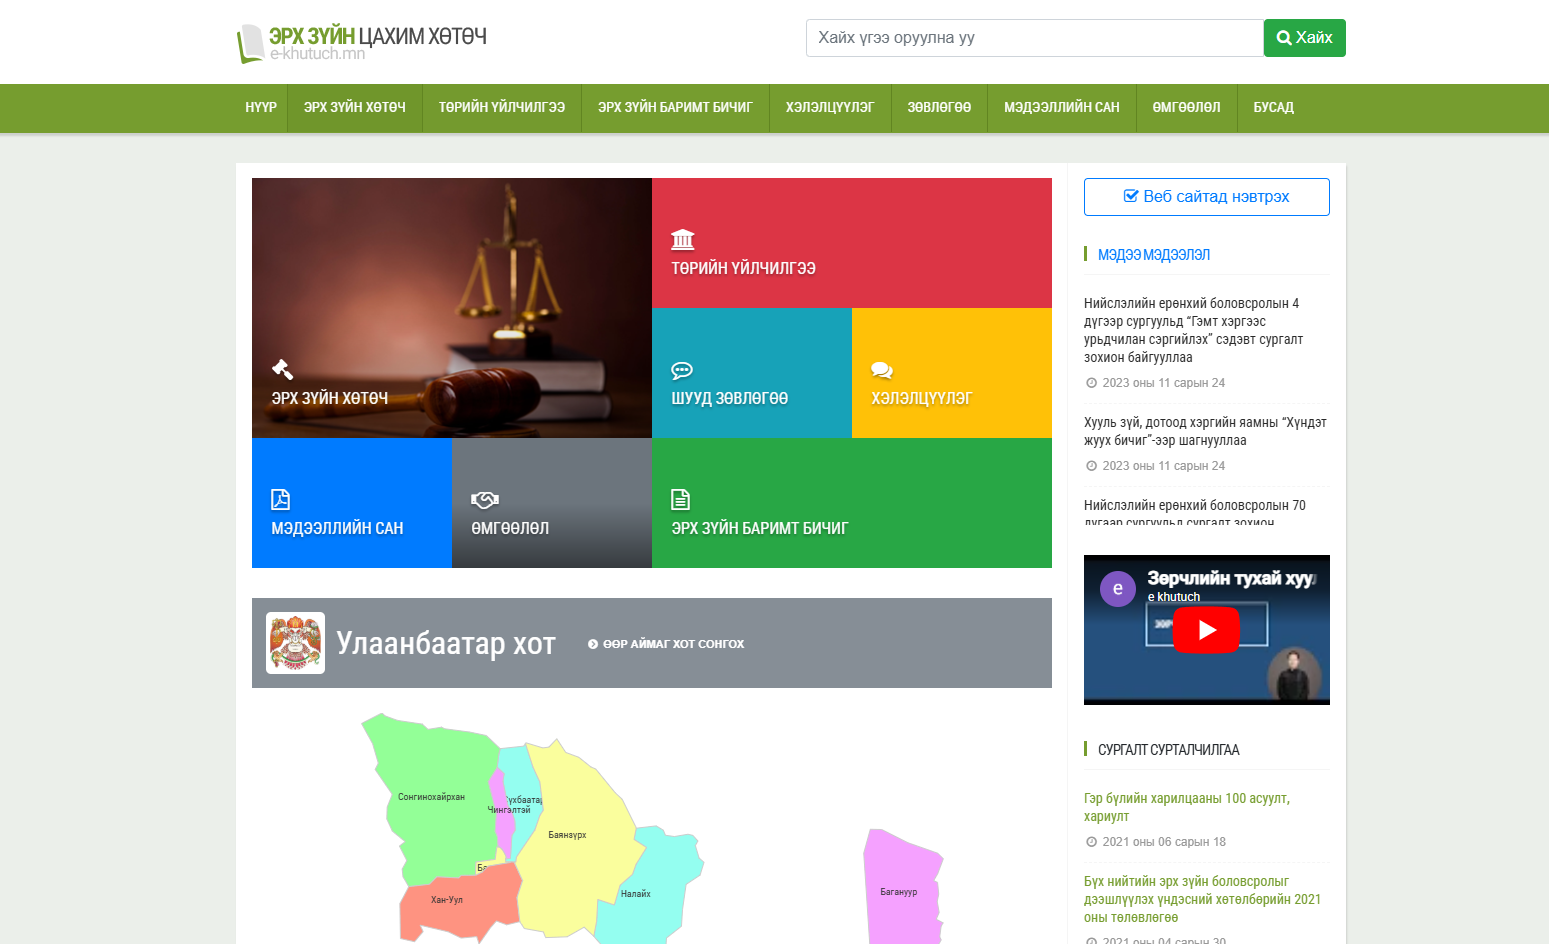
\includegraphics[scale=0.3]{Chart/Khutuch.png}
	\caption[E-khutuch нүүр хуудас]{E-khutuch.mn}
	\label{fig:Chart1}
\end{figure}
%-------------------------------------------------------------------------------
\section{Технологийн судалгаа}

Уг системийг хөгжүүлэхдээ орчин үеийн, өндөр гүйцэтгэлтэй, хиймэл оюунд суурилсан веб технологиудыг ашигласан. Систем нь \textbf{Frontend}, \textbf{Backend}, \textbf{Database}, \textbf{AI үйлчилгээ} гэсэн үндсэн бүрэлдэхүүн хэсгүүдээс тогтох ба эдгээр нь харилцан уялдаатайгаар ажиллаж, хэрэглэгчид хууль зүйн зөвлөгөө өгөх үндсэн үйл ажиллагааг хэрэгжүүлнэ. Энэхүү систем нь зөвхөн эрүүгийн эрх зүйн хүрээнд хязгаарлагдахгүй бөгөөд цаашид төрөл бүрийн хууль, эрх зүйн мэдээллийг нэгтгэн \textbf{бүрэн хууль зүйн зөвлөгөө өгөх} боломжтой байхаар архитектур нь зохион байгуулагдсан.

\subsection{Back-End хөгжүүлэлтэд ашиглах технологиуд}

\begin{itemize}

    \item \textbf{FastAPI:} Python хэл дээр суурилсан, өндөр хурдтай, асинхрон ажиллагааг дэмждэг орчин үеийн веб фреймворк.
    \begin{itemize}
        \item \textbf{Давуу тал:} REST API хөгжүүлэхэд хялбар, Pydantic-тэй нягт уялддаг, request/response өгөгдлийн бүтцийг автоматаар шалгах боломжтой.
        \item \textbf{Ач холбогдол:} Хэрэглэгчийн асуулгыг боловсруулах, хуулийн өгөгдөл хайх, AI үйлчилгээтэй холбогдох, чат харилцан ярианы өгөгдлийг хадгалах зэрэг үндсэн бизнес логикийг хэрэгжүүлдэг.
    \end{itemize}

    \item \textbf{Uvicorn:} FastAPI програмыг ажиллуулах ASGI сервер.
    \begin{itemize}
        \item \textbf{Ач холбогдол:} Асинхрон хүсэлтүүдийг үр ашигтай боловсруулж, системийн хурд болон хариу өгөх чадварыг нэмэгдүүлдэг.
    \end{itemize}

    \item \textbf{Pydantic:} Өгөгдлийн шалгалт, сериалчлал хийх сан.
    \begin{itemize}
        \item \textbf{Ач холбогдол:} API руу орж ирж буй болон буцаж буй өгөгдлийн бүтэц, төрлийг нарийн хянах боломж олгодог.
    \end{itemize}

    \item \textbf{Pydantic-Settings:} Орчны хувьсагч болон системийн тохиргоог удирдах сан.
    \begin{itemize}
        \item \textbf{Ач холбогдол:} API key, database URL зэрэг нууц болон орчны тохиргоог аюулгүй байдлаар удирддаг.
    \end{itemize}

    \item \textbf{Python:} Хиймэл оюун, өгөгдөл боловсруулах, backend хөгжүүлэлтийн өргөн хэрэглээтэй програмчлалын хэл.
    \begin{itemize}
        \item \textbf{Ач холбогдол:} Хуулийн текст боловсруулах, PDF-ээс өгөгдөл ялгах, API логик боловсруулах үндсэн хөгжүүлэлтийн орчин болж ажилладаг.
    \end{itemize}

\end{itemize}

\subsection{Өгөгдлийн сангийн түвшинд ашиглах технологиуд}

\begin{itemize}

    \item \textbf{PostgreSQL:} Системийн үндсэн харилцаат өгөгдлийн сан.
    \begin{itemize}
        \item \textbf{Давуу тал:} Найдвартай, өргөтгөх боломжтой, бүтэцтэй өгөгдөл хадгалахад тохиромжтой.
        \item \textbf{Ач холбогдол:} Хэрэглэгчийн бүртгэл, чат кейсүүд, мессежүүд, хуулийн ангилал болон хуулийн зүйл заалтуудыг хадгалдаг.
    \end{itemize}

    \item \textbf{Neon Cloud:} PostgreSQL өгөгдлийн санг клауд орчинд байршуулсан үйлчилгээ.
    \begin{itemize}
        \item \textbf{Ач холбогдол:} Өгөгдлийн санг алсын сервер дээр найдвартай байршуулж, хөгжүүлэлт болон ашиглалтын үеийн уян хатан байдлыг хангадаг.
    \end{itemize}

    \item \textbf{SQLAlchemy 2.0:} ORM буюу өгөгдлийн сантай обьект хандлагат аргаар ажиллах сан.
    \begin{itemize}
        \item \textbf{Ач холбогдол:} PostgreSQL хүснэгтүүдийг Python класс байдлаар тодорхойлж, өгөгдөлтэй илүү ойлгомжтой, эмх цэгцтэй ажиллах боломж олгодог.
    \end{itemize}

    \item \textbf{Alembic:} Өгөгдлийн сангийн schema хувилбар удирдах хэрэгсэл.
    \begin{itemize}
        \item \textbf{Ач холбогдол:} Хүснэгтийн бүтэц өөрчлөгдөх үед migration үүсгэж, database schema-г хяналттай шинэчлэх боломж бүрддэг.
    \end{itemize}

    \item \textbf{asyncpg / psycopg / aiosqlite:} PostgreSQL болон SQLite-д холбогдох драйверууд.
    \begin{itemize}
        \item \textbf{Ач холбогдол:} asyncpg нь асинхрон ажиллагаанд, psycopg нь өгөгдөл импортлох зэрэг тусгай скриптүүдэд, aiosqlite нь хөгжүүлэлтийн орчинд нөөц хувилбараар ашиглагддаг.
    \end{itemize}

\end{itemize}

\subsection{Хэрэглэгчийн баталгаажуулалт ба аюулгүй байдлын технологиуд}

\begin{itemize}

    \item \textbf{python-jose:} JWT токен үүсгэх болон шалгах сан.
    \begin{itemize}
        \item \textbf{Ач холбогдол:} Хэрэглэгчийн нэвтрэлт, session баталгаажуулалтыг хэрэгжүүлдэг.
    \end{itemize}

    \item \textbf{passlib + bcrypt:} Нууц үгийг hash хэлбэрээр аюулгүй хадгалах сангууд.
    \begin{itemize}
        \item \textbf{Ач холбогдол:} Хэрэглэгчийн нууц үгийг энгийн текстээр хадгалахгүй, bcrypt алгоритмаар hash хийж өгөгдлийн санд бичдэг.
    \end{itemize}

    \item \textbf{CORS Middleware:} Cross-Origin хүсэлтийг зохицуулах middleware.
    \begin{itemize}
        \item \textbf{Ач холбогдол:} Frontend болон Backend тусдаа орчинд ажиллах үед аюулгүй өгөгдөл солилцох нөхцөлийг бүрдүүлдэг.
    \end{itemize}

\end{itemize}

\subsection{Front-End хөгжүүлэлтэд ашиглах технологиуд}

\begin{itemize}

    \item \textbf{Next.js (React Framework):} Орчин үеийн frontend framework.
    \begin{itemize}
        \item \textbf{Давуу тал:} Хурдан, зохион байгуулалт сайтай, хэрэглэгчийн интерфэйсийг динамик байдлаар хөгжүүлэх боломжтой.
        \item \textbf{Ач холбогдол:} Хэрэглэгч асуулт оруулах, хариулт харах, кейсийн түүх үзэх, профайл мэдээллээ удирдах зэрэг интерфэйсийн үндсэн ажиллагааг хэрэгжүүлдэг.
    \end{itemize}

    \item \textbf{Tailwind CSS болон Shadcn UI:} Хэрэглэгчийн интерфэйсийн загварчлалын сангууд.
    \begin{itemize}
        \item \textbf{Ач холбогдол:} Системийн интерфэйсийг цэвэрхэн, ойлгомжтой, орчин үеийн харагдуулахад ашигладаг.
    \end{itemize}

    \item \textbf{Lucide React:} Дүрс тэмдэгтийн сан.
    \begin{itemize}
        \item \textbf{Ач холбогдол:} Системийн товч, цэс, үйлдлүүдийг ойлгомжтой дүрслэхэд хэрэглэгддэг.
    \end{itemize}

\end{itemize}

\subsection{AI интеграцчилалд ашиглах технологиуд}

\begin{itemize}

    \item \textbf{Google Gemini 2.5 Flash:} Хууль зүйн асуултад боловсруулалт хийх үндсэн хиймэл оюуны загвар.
    \begin{itemize}
        \item \textbf{Онцлог:} Хэрэглэгчийн асуулт болон өгөгдлийн сангаас олдсон хуулийн зүйл, заалтыг нэгтгэн хэлний боловсруулалт хийж, ойлгомжтой хариулт үүсгэдэг.
        \item \textbf{Ач холбогдол:} Системийн AI зөвлөх хэсгийг бүрдүүлж, хэрэглэгчид хууль зүйн асуултад тайлбарласан, утгын хувьд боловсруулсан хариулт өгдөг.
    \end{itemize}

    \item \textbf{httpx:} Асинхрон HTTP client сан.
    \begin{itemize}
        \item \textbf{Ач холбогдол:} Backend-ээс Gemini API руу хүсэлт илгээж, AI хариултыг асинхрон байдлаар хүлээн авахад ашиглагддаг.
    \end{itemize}

    \item \textbf{OpenAI-compatible API format:} Chat completion бүтэцтэй API хүсэлтийн формат.
    \begin{itemize}
        \item \textbf{Ач холбогдол:} Gemini загвартай стандартчилсан хэлбэрээр холбогдож, системийг цаашид өөр төрлийн ижил төстэй AI загваруудтай холбох уян хатан боломж бүрддэг.
    \end{itemize}

\end{itemize}

\subsection{Хуулийн баримт бичиг боловсруулах технологиуд}

\begin{itemize}

    \item \textbf{PyMuPDF (fitz):} PDF файлуудаас текст задлан авах сан.
    \begin{itemize}
        \item \textbf{Ач холбогдол:} Хуулийн эх баримт бичгүүдээс текстийг автоматаар гарган авч, өгөгдлийн санд оруулах бэлтгэлийг хангадаг.
    \end{itemize}

    \item \textbf{Custom Parser:} Regex-д суурилсан тусгай боловсруулалтын логик.
    \begin{itemize}
        \item \textbf{Ач холбогдол:} Хуулийн бүлэг, зүйл, заалт, дэд заалтыг ялгаж танин, тэдгээрийг бүтэцтэй өгөгдөл болгон хадгалах боломж олгодог.
    \end{itemize}

\end{itemize}

%-------------------------------------------------------------------------------
\section{Өөрийн хөгжүүлж буй системийн онолын үндэслэл}

\subsection{Байгалийн хэл боловсруулалт (NLP) ба хууль зүйн текстийн боловсруулалт}

Систем нь хэрэглэгчийн энгийн хэлээр бичсэн асуултыг боловсруулж, өгөгдлийн санд хадгалагдсан хууль зүйн мэдээлэлтэй уялдуулан хариулт гаргах \textbf{байгалийн хэл боловсруулалт (Natural Language Processing, NLP)}-ын зарчимд суурилна. NLP нь хүний хэлийг компьютерт ойлгуулах, боловсруулах, утгыг нь тайлбарлах чиглэлийн шинжлэх ухааны салбар бөгөөд хэрэглэгчийн асуултын утгыг зөв тайлбарлах, холбогдох хуулийн заалтыг олж хэрэглэгчид ойлгомжтой хариулт бүрдүүлэхэд чухал үүрэг гүйцэтгэдэг. Хууль зүйн зөвлөгөө өгөхдөө зөвхөн нэг төрлийн хуульд бус, олон төрлийн хууль, эрх зүйн эх сурвалжийг хамруулан ашиглах боломжтойгоор зохион байгуулагдсан нь системийн онолын болон практик ач холбогдлыг нэмэгдүүлж байна.

\subsection{Мэдээлэл сэргээх ба AI тусламжтай хариулт боловсруулах зарчим (RAG)}

\subsubsection{RAG гэж юу вэ?}

\textbf{Retrieval-Augmented Generation (RAG)} буюу \textbf{мэдээлэл сэргээн нөхөн авах ба генерацлах} арга нь хиймэл оюуны хэлний загварыг гадаад мэдээллийн сантай хослуулан ашиглах архитектурын загвар юм. Уламжлалт хэлний загвар нь зөвхөн сургалтын үед олж авсан мэдлэгтээ тулгуурлан хариулт үүсгэдэг тул актуал бус буюу буруу мэдээлэл (``hallucination'') гаргах эрсдэлтэй байдаг. RAG загвар нь энэ дутагдлыг арилгахын тулд хариулт үүсгэхийн өмнө өгөгдлийн сангаас холбогдох мэдээллийг хайж олж, тэдгээрийг контекст болгон хэлний загварт дамжуулдаг.

RAG загварын үндсэн гурван үе шат:
\begin{enumerate}
    \item \textbf{Indexing (Индексжүүлэлт):} Хуулийн эх баримт бичгүүдийг боловсруулж, хайлтад бэлэн бүтэцтэй өгөгдөл болгон өгөгдлийн санд хадгална.
    \item \textbf{Retrieval (Мэдээлэл сэргээх):} Хэрэглэгчийн асуулттай утгын хувьд хамгийн ойр холбогдох хуулийн заалтуудыг өгөгдлийн сангаас хайж олно.
    \item \textbf{Generation (Хариулт үүсгэх):} Олдсон хуулийн мэдээлэл болон хэрэглэгчийн асуултыг нэгтгэн prompt үүсгэж, хиймэл оюуны загварт дамжуулснаар тайлбарласан, бодит эх сурвалжтай хариулт боловсруулна.
\end{enumerate}

\subsubsection{Системд RAG-ийг хэрхэн хэрэглэж байна}

Энэхүү систем нь хэрэглэгчийн асуултыг шууд AI загварт дамжуулах бус, эхлээд PostgreSQL өгөгдлийн сангаас холбогдох хууль, зүйл заалтыг хайж олсны дараа тэдгээрийг асуулттай нэгтгэн Google Gemini 2.5 Flash загварт өгч хариулт боловсруулдаг. Өөрөөр хэлбэл, хариулт нь зөвхөн ерөнхий хэлний загварын мэдлэгээс бус, системд хадгалагдсан Монгол Улсын хуулийн өгөгдөлд тулгуурлан үүсдэг. Энэ нь хариултын үндэслэл, бодит эх сурвалжтай байх нөхцөлийг хангаж, ``hallucination'' буюу буруу мэдээлэл гарах эрсдэлийг мэдэгдэхүйц бууруулдаг.

\subsection{Мэдээллийн системийн давхаргат архитектур (Layered Architecture)}

Систем нь Presentation Layer, Application Layer, Data Layer гэсэн давхаргат архитектурт тулгуурлан зохион байгуулагдсан.
\begin{itemize}
    \item \textbf{Presentation Layer:} Frontend интерфэйс, хэрэглэгчийн оролт ба хариултын дүрслэл.
    \item \textbf{Application Layer:} FastAPI backend, authentication, бизнес логик, AI интеграцчилал.
    \item \textbf{Data Layer:} PostgreSQL өгөгдлийн сан, хуулийн зүйл заалт, хэрэглэгч, кейс, мессежийн мэдээлэл.
\end{itemize}

Энэхүү давхаргат архитектур нь системийг модульчлагдсан, өргөтгөх боломжтой, засвар үйлчилгээ хийхэд хялбар болгодог. Тухайлбал, цаашид Иргэний хууль, Захиргааны хууль, Хөдөлмөрийн хууль зэрэг бусад хууль, эрх зүйн эх сурвалжийг нэмэхэд зөвхөн өгөгдлийн сангийн түвшинд өргөтгөл хийх байдлаар хөгжүүлэх боломжтой.

\subsection{Программ хангамжийн ёс зүй ба AI хариуцлага}

Хууль зүйн зөвлөгөө өгөх системийн хувьд AI-ийн хариултын үнэн зөв байдал, хэрэглээний эрсдэл нь онцгой ач холбогдолтой. Иймд систем нь AI-ийг дангаар нь шийдвэр гаргагч байдлаар ашиглахгүй, харин өгөгдлийн санд хадгалагдсан хууль зүйн эх сурвалжид тулгуурлан зөвлөмж боловсруулах туслах хэрэгсэл байдлаар ашигладаг. Энэ нь хиймэл оюуны ``hallucination'' эрсдэлийг бууруулж, хэрэглэгчид илүү бодитой, хариуцлагатай зөвлөгөө хүргэх үндэс болдог.

%-------------------------------------------------------------------------------
\section{Бүлгийн дүгнэлт}

Энэ бүлэгт хөгжүүлж буй хууль зүйн зөвлөх системийн технологийн болон онолын үндэслэлийг авч үзлээ. Тодруулбал, FastAPI, PostgreSQL, SQLAlchemy, JWT authentication, PDF текст задлалт, Google Gemini 2.5 Flash зэрэг технологиудыг ашиглан системийн backend, database, AI интеграцчиллыг хэрхэн хэрэгжүүлж байгааг тайлбарлав. Онолын хэсэгт NLP болон RAG загварын тухай тодорхойлж, уг систем нь бодит хуулийн өгөгдөлд тулгуурлан хариулт боловсруулдаг тул уламжлалт хэлний загвараас ялгарах давуу талыг дурдлаа. Мөн систем нь зөвхөн эрүүгийн эрх зүйгээр хязгаарлагдахгүй, харин олон төрлийн хууль, эрх зүйн эх сурвалжид тулгуурлан бүрэн хууль зүйн зөвлөгөө өгөх боломжтой давхаргат архитектуртай болохыг онолын түвшинд үндэслэн тайлбарлалаа.